\chapter{Desenvolvimento}
\label{methodology}

  \section{Dispositivos utilizados} 
  \label{methodology:devices}

    \subsection{BeagleBone Black e OSSO Cape} 
    \label{methodology:devices:bbb}

      A BeagleBone Black é uma placa de desenvolvimento \textit{open-source}, desenvolvida pela \textit{Texas Instruments}, do tamanho aproximado de um cartão de crédito. Embora possua um tamanho reduzido, possui os recursos de hardware necessários para viabilizar a execução de distribuições \textit{Linux} como, por exemplo, o Debian (que foi a utilizada nesse projeto).

      \begin{figure}[H]
        \begin{center}
          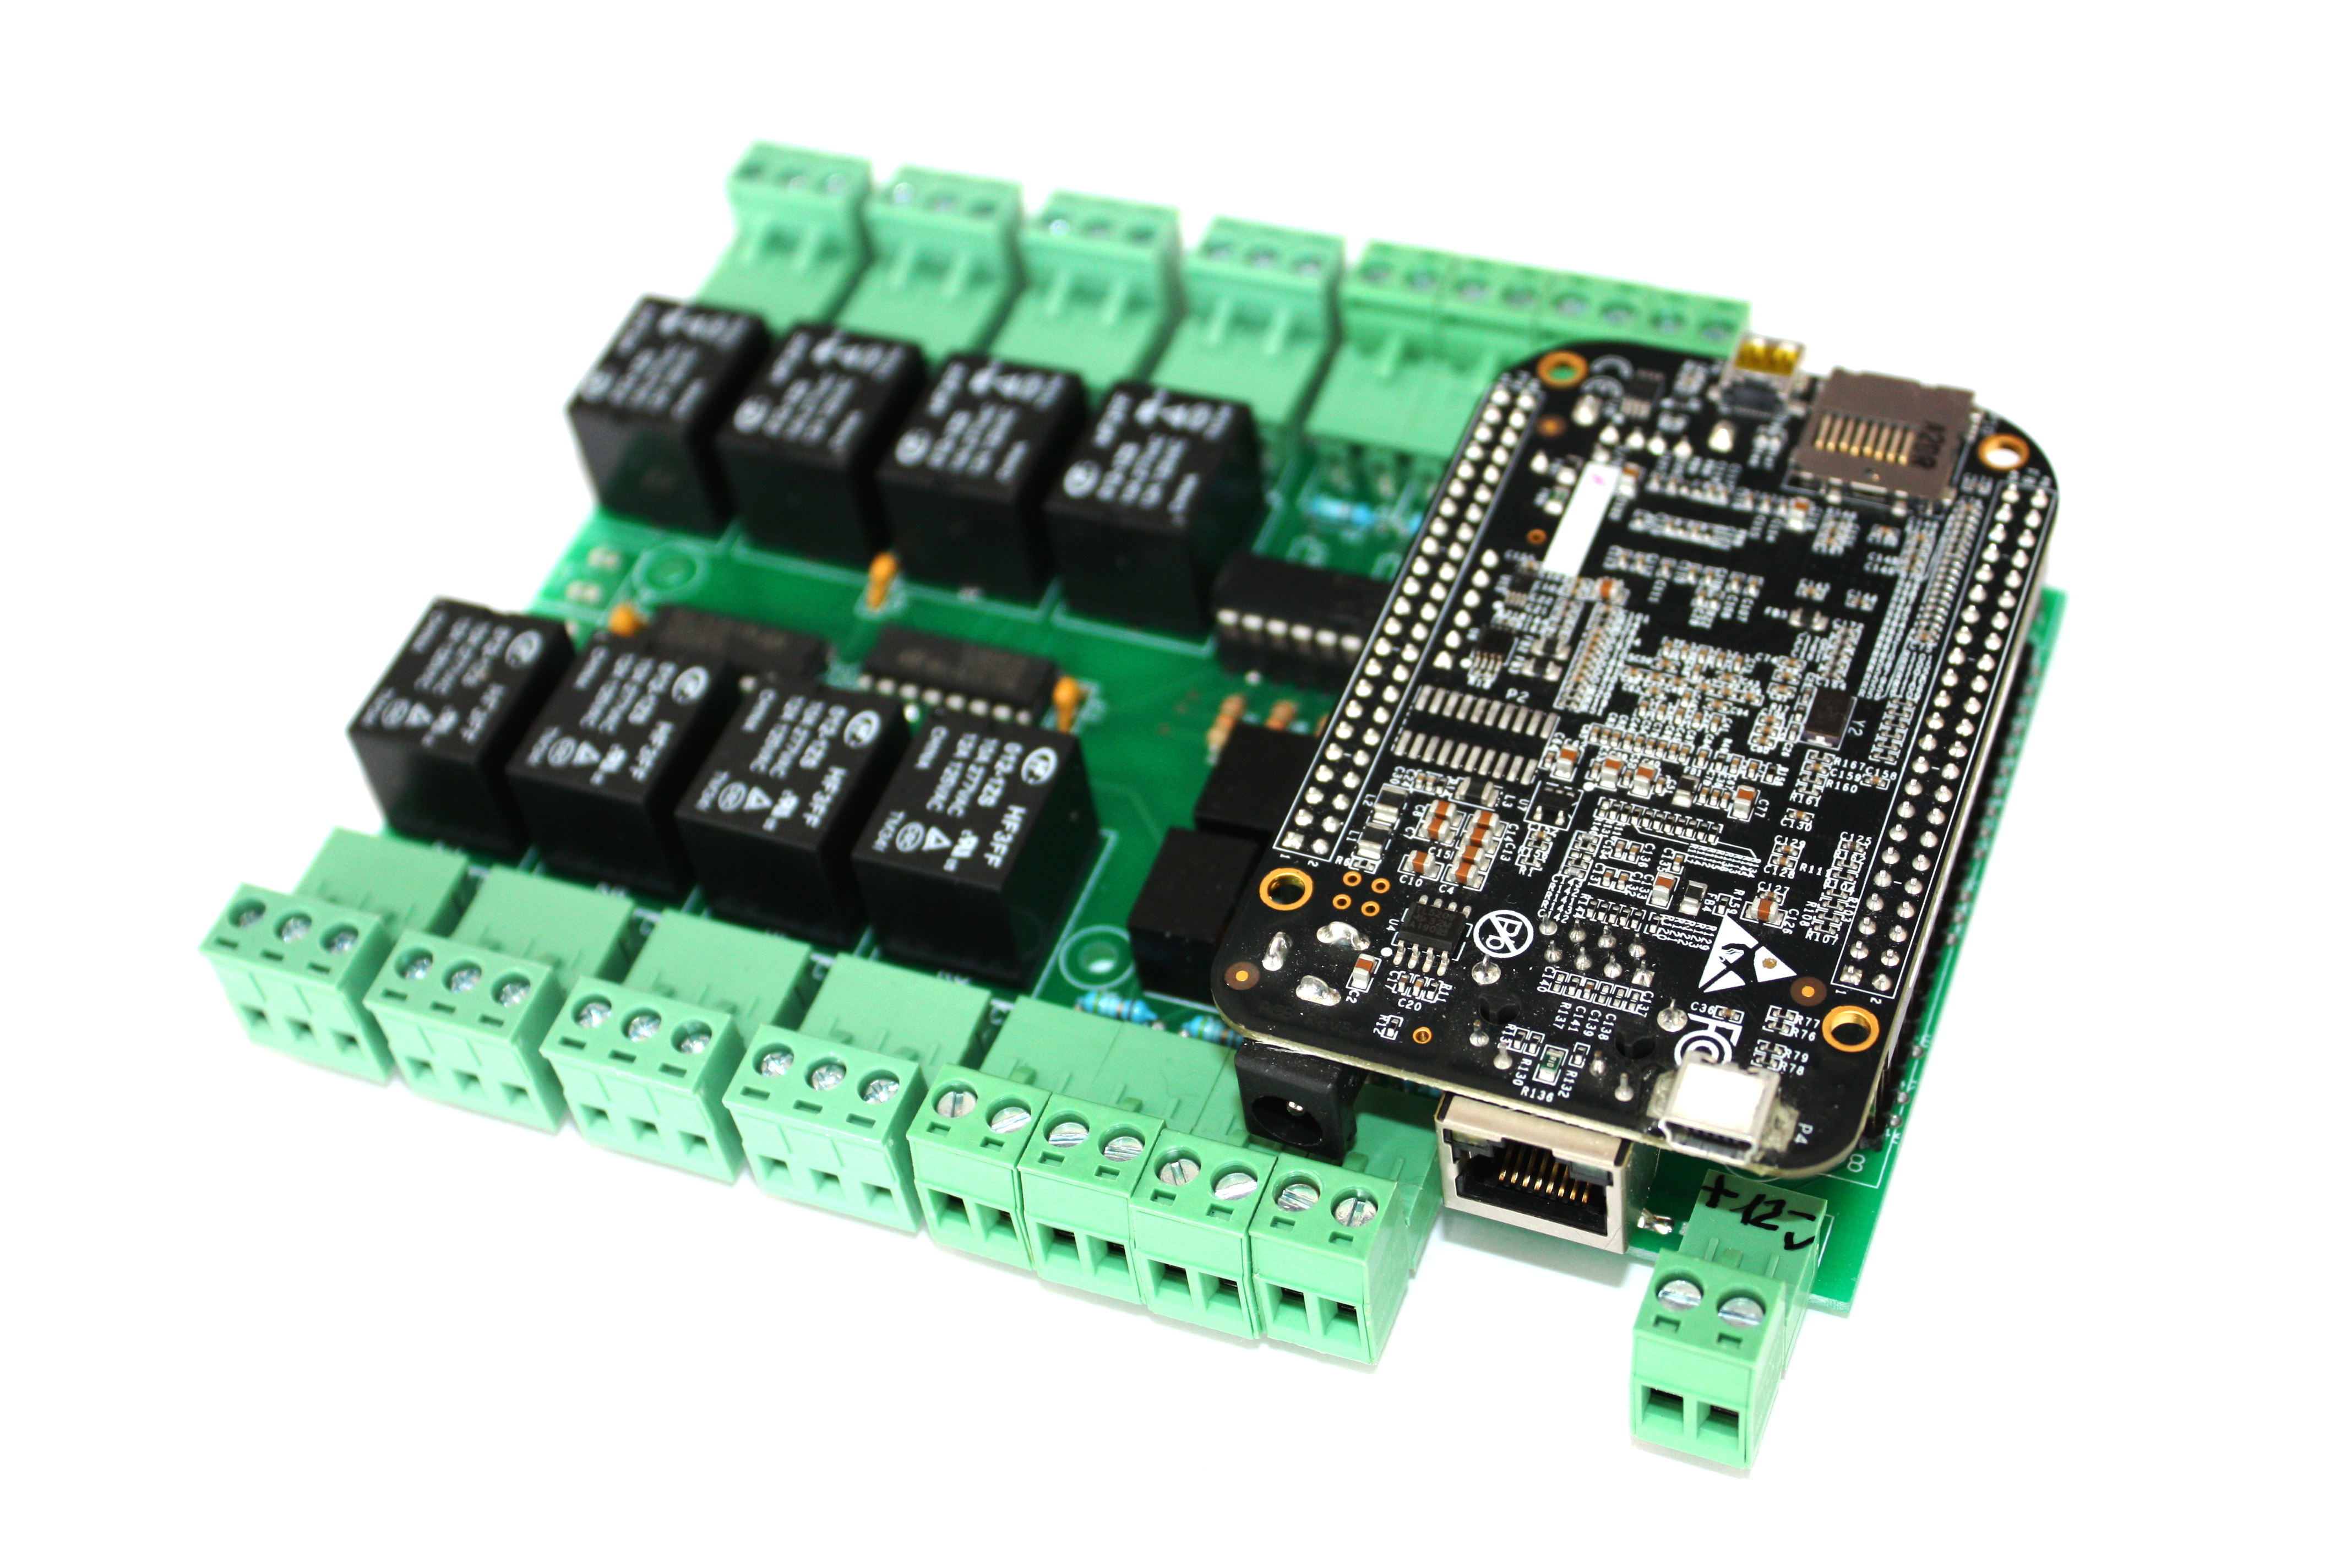
\includegraphics[width=0.75\textwidth,natwidth=585,natheight=180]{assets/images/devices-beaglebone.jpg}
          \caption{BeagleBone Black e OSSO Cape}
          \label{fig:bbb}
        \end{center}
      \end{figure}

      A BeagleBone permite expansões por meio de \textit{capes}, placas não-oficiais que permitem melhor explorar o uso das saídas e entradas. Nesse projeto, foi utilizada a OSSO Cape, que dispõe de:

      \begin{itemize}
        \item Oito entradas digitais opto-acopladas
        \item Oito saídas digitais por meio de relés
        \item Porta RS-485 integrada
        \item Porta I2C integrada
        \item Alimentação de fontes externas com tensões entre 5 à 24V
      \end{itemize}

      A utilização da cape permite um uso fácil das entradas e saídas digitais, assim como da comunicação RS-485. Caso não fosse utilizada, seria necessário planejar e fabricar uma placa com as proteções e acionamentos que necessários para as entradas e saídas, assim como montar um circuito para converter a saída \ac{UART} para RS-485. 

    \subsection{Medidor de Energia Kron Mult-K}
    \label{methodology:devices:kron}

      O medidor de energia é essencial para informar tanto ao usuário, quanto ao sistema central, quanta energia foi consumida durante os carregamentos. O dispositivo escolhido foi o Kron Mult-K, pois esse permite a medição da energia consumida e outros dados, todos disponibilizados via MODBUS-RTU (conexão RS-485).

      \begin{figure}[H]
        \begin{center}
          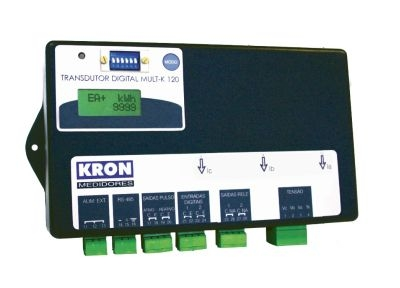
\includegraphics[width=0.75\textwidth,natwidth=400,natheight=288]{assets/images/devices-kron.jpg}
          \caption{Medidor Kron da série Mult-K}
          \label{fig:kron}
        \end{center}
      \end{figure}

    \subsection{Phoenix EM-CP-PP-ETH Controller}
    \label{methodology:devices:phoenix}

      Os padrões de carregamento rápido utilizam protocolos de comunicação entre carro e estação, podendo ser via \textit{\ac{PWM}} ou \textit{\ac{CAN}}. O Phoenix EM-CP-PP-ETH permite gerenciar carregamentos AC trifásicos por meio do \textit{\ac{PWM}} e variação dos níveis de tensão, o que permite realizar todo controle necessário entre a inicialização e finalização dos carregamentos \cite{phoenix}. 

      Na figura \ref{fig:phoenix}, é possível ver um exemplo do sequenciamento de um carregamento gerenciado pelo Phoenix. No estado A, quando não há nada conectado, o conector apresenta uma saída de 12V constante. Assim que o veículo é conectado, a tensão cai para 9V e o estado muda para B. 

      Enquanto se manter em 9V constante (estado B1), a estação ainda não está pronta para o carregamento, porém assim que começar a se comunicar via \textit{\ac{PWM}} (estado B2), a estação indica que está pronta. A tensão então cai para 6V ou 3V (estado C ou D) e o veículo inicia o carregamento. A corrente fornecida é indicada pelo valor do \textit{\ac{PWM}}. 

      Ao termino do carregamento, o veículo desativa a PWM e a estação volta para o estado B. Após o conector ser removido pelo usuário, a estação vai para o estado A e permanece assim até o próximo carregamento.

      \begin{figure}[H]
        \begin{center}
          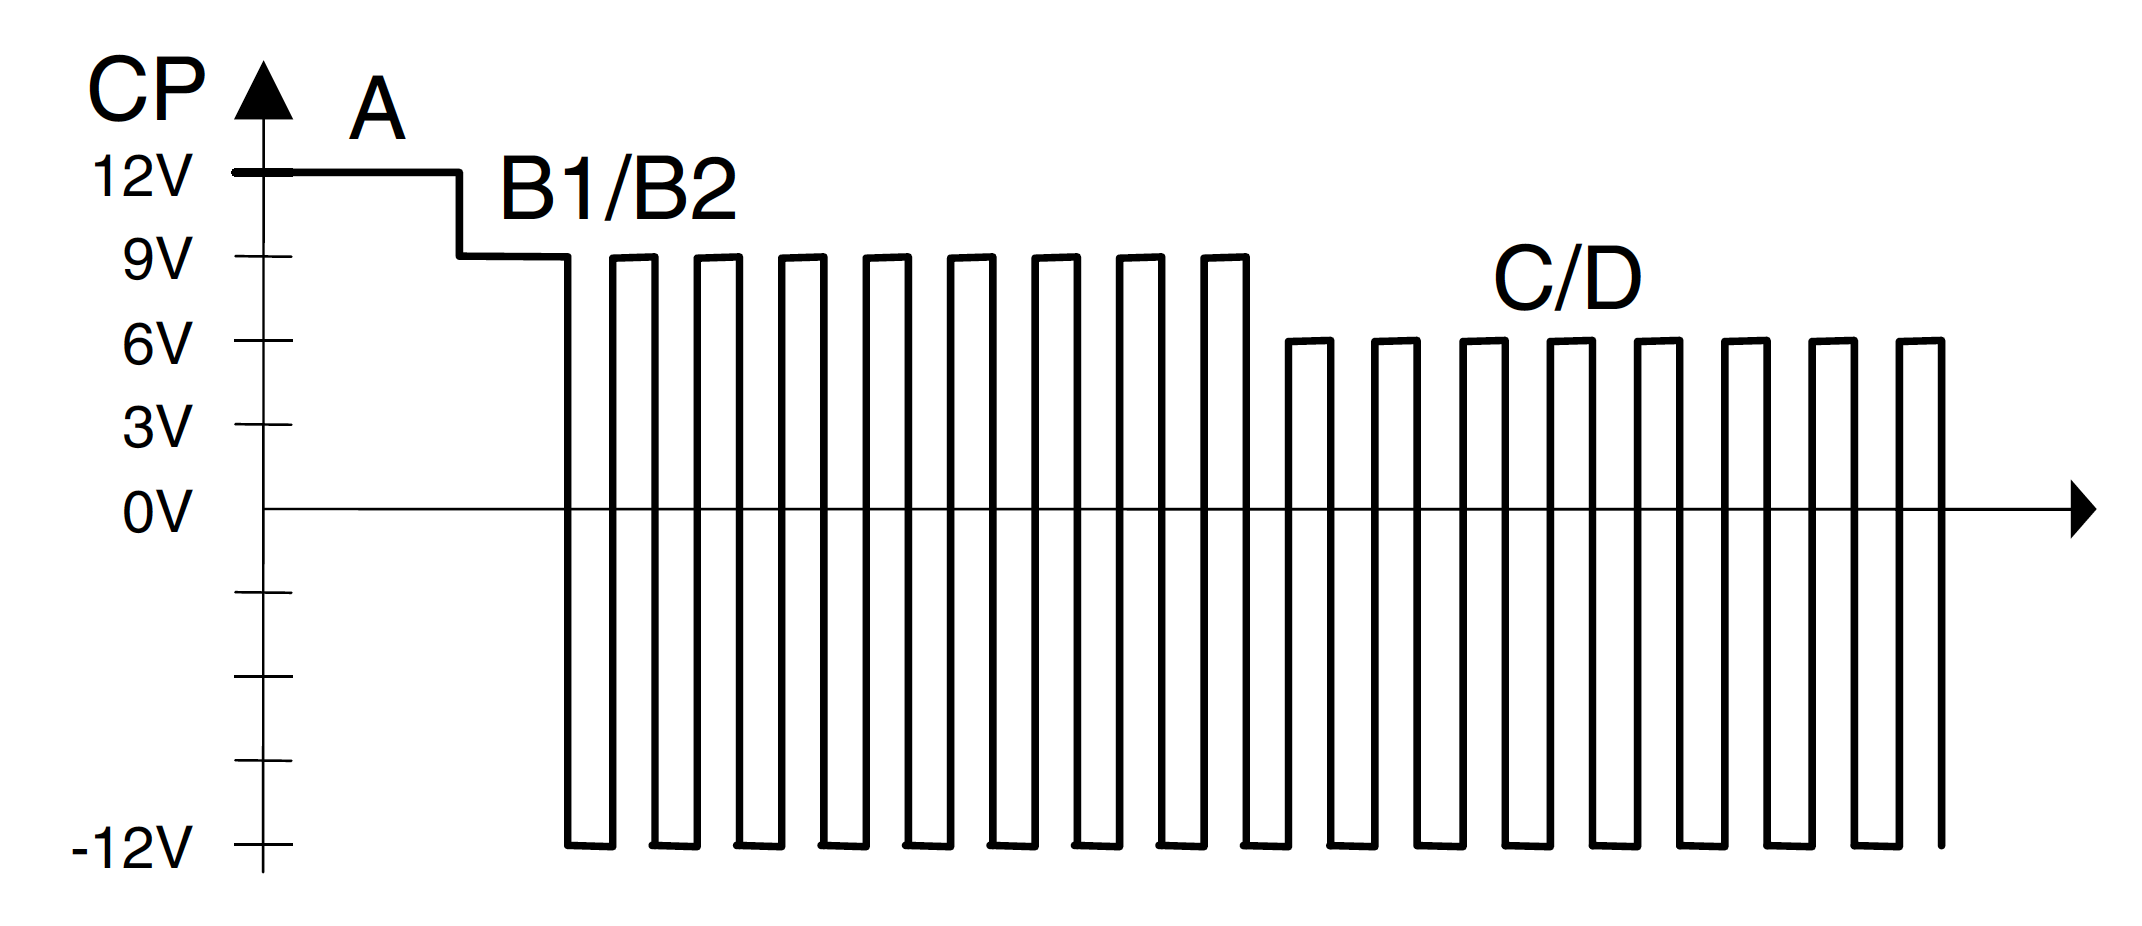
\includegraphics[width=0.75\textwidth,natwidth=400,natheight=288]{assets/images/phoenix.jpg}
          \caption{Exemplo de sequenciamento do Phoenix}
          \label{fig:phoenix}
        \end{center}
      \end{figure}

    \subsection{IHM WEG MT}
    \label{methodology:devices:ihm}

      Para o usuário utilizar a \ac{EVSE}, é necessária uma interface que apresente informações de forma descomplicada e, além disso, seja robusta a intempéries como calor excessivo e chuva. Para tal, foi escolhida a \ac{IHM} da WEG, linha MT.

      Utilizando o \textit{software EasyBuilder 8000}, é possível definir as telas que serão exibidas para o usuário, assim como os dados que serão exibidos. Os dados e o controle da IHM podem ser realizados por meio de diversos protocolos, dentre eles o MODBUS-TCP, o qual foi escolhido para o projeto.

      \begin{figure}[H]
        \begin{center}
          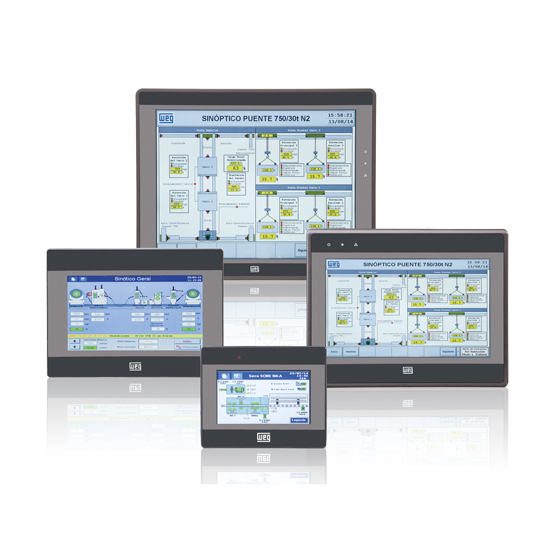
\includegraphics[width=0.75\textwidth,natwidth=400,natheight=288]{assets/images/devices-hmi.jpg}
          \caption{Linha de IHMs MT da WEG}
          \label{fig:ihm}
        \end{center}
      \end{figure}

    \subsection{Leitor de RFID LotusSmart}
    \label{methodology:devices:rfid}

      De acordo com a especificação do \textit{\ac{OCPP}}, para iniciar o carregamento na estação é necessária a utilização de cartões \textit{\ac{RFID}}, sendo necessário a utilização de um leitor compatível. O dispositivo escolhido, \textit{LotusSmart}, permite apenas a leitura de cartões de 13,56 MHz, visto que há uma variedade de frequências de operação.

      Os dados da \textit{tag} são armazenados em um \textit{buffer}, semelhante ao \textit{buffer} de teclado de computadores, e enviados serialmente para o sistema, sendo entregues em formato \textit{ASCII}.

      \begin{figure}[H]
        \begin{center}
          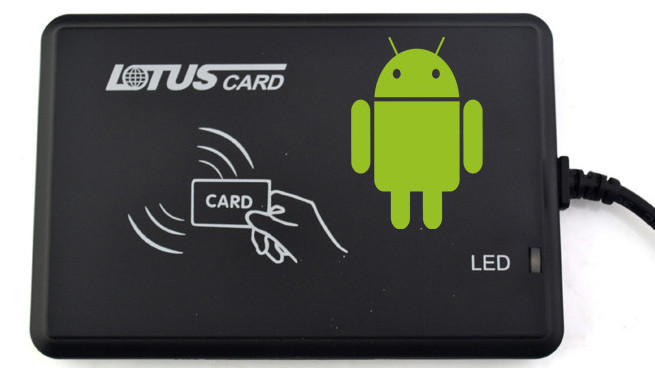
\includegraphics[width=0.75\textwidth,natwidth=655,natheight=368]{assets/images/devices-rfid.jpg}
          \caption{Leitor RFID LotusSmart}
          \label{fig:rfid}
        \end{center}
      \end{figure}

  \section{Métodos e Ferramentas utilizadas}
  \label{methodology:tools}

    \subsection{MODBUS}
    \label{methodology:tools:modbus}

      Em projetos industriais, é requisito que dispositivos diversos consigam comunicar-se entre si. Para tal, existem dezenas de protocolos que permitem a realização dessa tarefa, sendo o MODBUS um dos mais comuns \cite{modbus-spec-application}. Sua implementação inicial era apenas no modo serial, porém hoje também é possível utilizar o stack TCP/IP e outras implementações menos comuns - UDP, PEMEX, Enron.

      \subsubsection{Funcionamento}
      \label{methodology:tools:modbus:how}

        O protocolo é baseado no modelo mestre-escravo, onde um dispositivo mestre requisita os dados dos dispositivos escravos.

        \begin{figure}[H]
          \begin{center}
            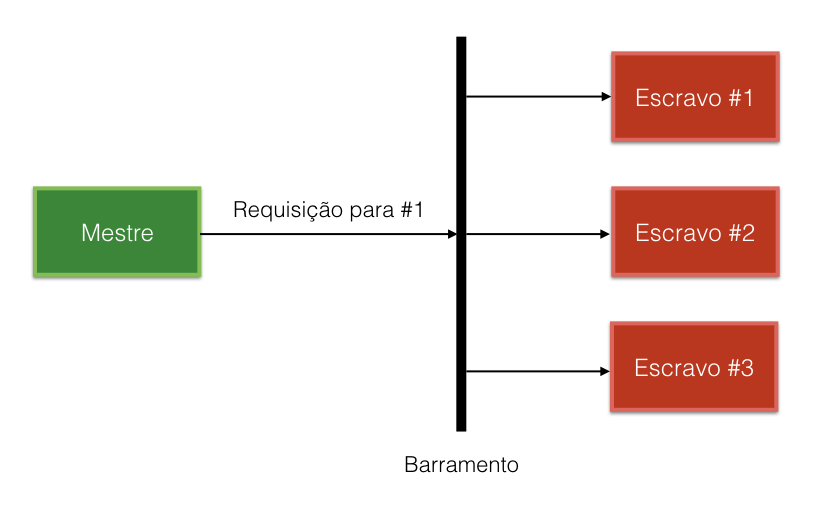
\includegraphics[width=0.8\textwidth,natwidth=1024,natheight=768]{assets/images/modbus-req-1.png}
            \caption{Requisição MODBUS do mestre para o escravo}
            \label{fig:modbus-req-1}
          \end{center}
        \end{figure}

        Como uma rede pode ter N escravos, cada escravo possui um endereço atribuído. O mestre envia a requisição para o barramento e todos os escravos a recebem, porém somente o endereçado responderá. Há também a opção de se fazer um \textit{broadcast} - endereço 0 - onde todos escravos recebem a requisição, porém nesse caso nenhum escravo deve responde-lá.

        Vale notar que em uma rede MODBUS-RTU há somente um mestre, enquanto em uma rede MODBUS-TCP é possível que cada mestre seja um escravo, e vice-versa.

        \begin{figure}[H]
          \begin{center}
            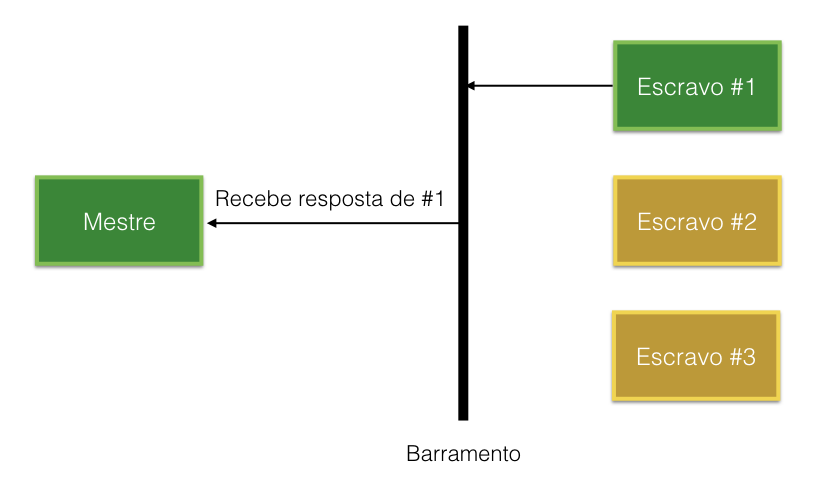
\includegraphics[width=0.8\textwidth,natwidth=1024,natheight=768]{assets/images/modbus-req-2.png}
            \caption{Resposta MODBUS do escravo para o mestre}
            \label{fig:modbus-req-2}
          \end{center}
        \end{figure}

      \subsubsection{Mapa de Memória}
      \label{methodology:tools:modbus:memorymap}

        Toda requisição realizada pelo mestre endereçará um dado no mapa de memória do dispositivo escravo, sendo que tal mapa de memória normalmente deve ser indicado por uma documentação. Os dados requisitados podem possuir quatro tipos distintos:

        \begin{itemize}
          \item \textit{Input}: dado binário que permite apenas leitura
          \item \textit{Coil}: dado binário que permite leitura e escrita
          \item \textit{Input Register}: registrador com 16 bits (inteiro) que permite apenas leitura
          \item \textit{Holding} Register: registrador com 16 bits (inteiro) que permite leitura e escrita
        \end{itemize}

        Para a realização de operações nesse mapa de memória, o mestre precisa informar nas suas requisições um \textit{function code}. Este indicará qual dado deseja-se requisitar e se será executada uma operação de leitura ou escrita. A tabela \ref{table:modbus-funccodes} mostra os mais comuns, porém existem mais códigos, aos quais podem ser usados para diagnósticos e entre outras funções.

        \begin{table}[]
          \centering
          \caption{Function codes / Operações do MODBUS}
          \label{table:modbus-funccodes}
          \begin{tabular}{@{}ll@{}}
            \toprule
            \textbf{Operação}              & \textbf{Function code} \\ \midrule
            Leitura de Coils               & 1                      \\
            Escrita em 1 Coils             & 5                      \\
            Escrita em N Coils             & 15                     \\
            Leitura de Inputs              & 2                      \\
            Leitura de Input Registers     & 4                      \\
            Leitura de Holding Registers   & 3                      \\
            Escrita em 1 Holding Register  & 6                      \\
            Escrita em N Holding Registers & 16                     \\ \bottomrule
          \end{tabular}
        \end{table}

      \subsubsection{Envio de informações}
      \label{methodology:tools:modbus:frame}

        Cada modo possui alguma diferença, porém o meio que as informações são organizadas e enviadas é o mesmo. Na figura \ref{fig:modbus-frame} é possível observar que em ambas implementações é necessária a definição de um \textit{FCode (function code)}. Logo após vem o campo \textit{Data}, onde devem ser indicados o endereço inicial do mapa de memória, quantos registradores deseja-se requisitar e quais dados serão escritos (no caso de escrita).

        \begin{figure}[H]
          \begin{center}
            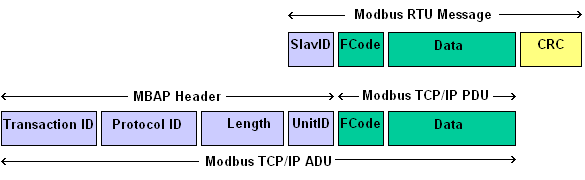
\includegraphics[width=\textwidth,natwidth=585,natheight=180]{assets/images/modbus-frame.png}
            \caption{Frame de Comunicação MODBUS}
            \label{fig:modbus-frame}
          \end{center}
        \end{figure}

        Como pode-se notar, no MODBUS-RTU há o SlavID, que é utilizado para endereçar qual dispositivo se deseja requisitar (endereço). No MODBUS-TCP há o UnitID, que funciona para a mesma finalidade que o SlavID, e pode ser utilizado em conjunto com o endereço IP do dispositivo. O campo CRC é um dado que permite checar se o pacote obtido possui ou não algum erro. Como o protocolo TCP/IP já possui um meio para isso, tal campo não é incluído na requisição.

        Esse formato de envio de informações é mantido tanto para requisição quanto para resposta, sendo que as respostas sempre possuem o mesmo \textit{function code} da requisição. Caso diferir, provavelmente ocorreu um erro e este pode ser processado pelo mestre posteriormente.

    \subsection{WSDL e SOAP}
    \label{methodology:tools:wsdlsoap}

      O WSDL \cite{w3c-spec-wsdl} permite descrever serviços web por meio de um arquivo \textit{\ac{XML}}. É possível definir os \textit{endpoints} - pontos de entrada para requisições - com o que devem retornar e o que devem receber como parâmetros. Isso permite que um serviço \textit{web} seja desenvolvido por uma equipe que, posteriormente, exporta um \textit{\ac{WSDL}} descrevendo de maneira fácil quais são seus \textit{endpoints}, o que facilita a criação de clientes ou servidores compatíveis com o serviço.

      Os arquivos WSDL definem suas interfaces em \textit{\ac{SOAP}} \cite{w3c-spec-soap}, um protocolo que permite trocas de informações entre clientes e servidores de forma padronizada. Sendo baseado em \textit{\ac{XML}}, é montado em três partes:
      \begin{itemize}
        \item Envelope: identifica o que é a mensagem e como processá-la
        \item Cabeçalho: define informações extras sobre a mensagem
        \item Corpo: define o procedimento a ser chamado e os dados de sua resposta
      \end{itemize}

      Como o \textit{\ac{WSDL}} foi idealizado em \textit{\ac{XML}}, é facilmente processado por qualquer linguagem de programação, o que garante uma boa portabilidade.

    \subsection{JUnit e Automação de testes}
    \label{methodology:tools:junit}

      O \textit{JUnit} é um \textit{framework} que facilita a criação de código para a automação de testes unitários. Pode ser verificado se cada método de uma classe funciona da forma esperada, identificando possíveis erros antes de ser enviado para o ambiente de produção (exemplo: servidor ou placa de desenvolvimento) \cite{developer-junit}.

      Isso é de extrema importância para casos onde a equipe precisa modificar diversas classes, porém precisa manter suas funcionalidades. Assim, caso alguma modificação gerar alguma falha durante os testes, o desenvolvedor rapidamente poderá analisar e corrigir a falha, não deixando esta se propagar no meio de produção, minimizando a chance de \textit{bugs}.

      Um dos problemas da utilização de \textit{frameworks} de automação de teste é a exigência de uma boa dedicação para a criação dos testes, algo nem sempre possível devido a limitações de projeto, como prazos de entrega. Outro é a necessidade de uma boa experiência para a criação de testes úteis e assertivos, pois é necessário um balanço entre quanto tempo dedicar e quais funcionalidades são críticas (e devem ser testadas). Além disso, o ideal seria que um terceiro instrumentasse as classes utilizando o \textit{framework}, e não o desenvolvedor, pois este estará viciado em seu código, enquanto um terceiro procurará por situações não observados pelo desenvolvedor.

    \subsection{Guice e Injeção de Dependências}
    \label{methodology:tools:guice}

      A injeção de dependências permite que as classes sejam pouco acopladas entre si. Para tal, a lógica de instanciação das dependências não é gerenciada pela classe que as utiliza. O desenvolvedor só necessitará declarar quais dependências (outras classes) deseja e se preocupar em como utilizá-las na classe.

      A tarefa de instanciação e injeção dessas dependências é feita por um \textit{service container}, retirando a responsabilidade das instanciações das classes (o que as torna menos acopladas). Existem algumas ferramentas disponíveis que implementam isso de forma eficiente, como o \textit{Guice} e o \textit{Spring} \cite{developer-guice}. A escolhida foi o \textit{Guice}, desenvolvida e mantida pelo \textit{Google}.

  \section{Estrutura do Projeto}
  \label{methodology:structure}

    A figura \ref{fig:proj-diagram} apresenta o diagrama de conexão dos dispositivos. Como todos os dispositivos são compatíveis com MODBUS, esse foi o protocolo escolhido para a comunicação entre eles. Para a comunicação entre servidor e estação, foi escolhido o protocolo \ac{OCPP} 1.5. 

    O \textit{software} foi desenvolvido em \textit{Java}, visto a facilidade para implementar uma \textit{API} \textit{\ac{SOAP}} a partir de um \textit{\ac{WSDL}}, o conhecimento de outros membros do projeto sobre a linguagem, a quantidade de recursos de suporte na web e a portabilidade fácil do código.

    A estação possui dois medidores, sendo um para o conector modo 2 (Med. Kron \#1) e outro para o conector \textit{Mennekes} - modo 3 (Med. Kron \#2). O controle de cada conector se dá de forma diferente: o de conector \textit{Mennekes} modo 3 utiliza o controlador \textit{Phoenix}, enquanto o conector modo 2 é controlado pela \textit{BeagleBone} e um relé, visto que esse é somente uma tomada comum e não necessita de nada muito elaborado para inicializar carregamentos.

    \begin{figure}[H]
      \begin{center}
        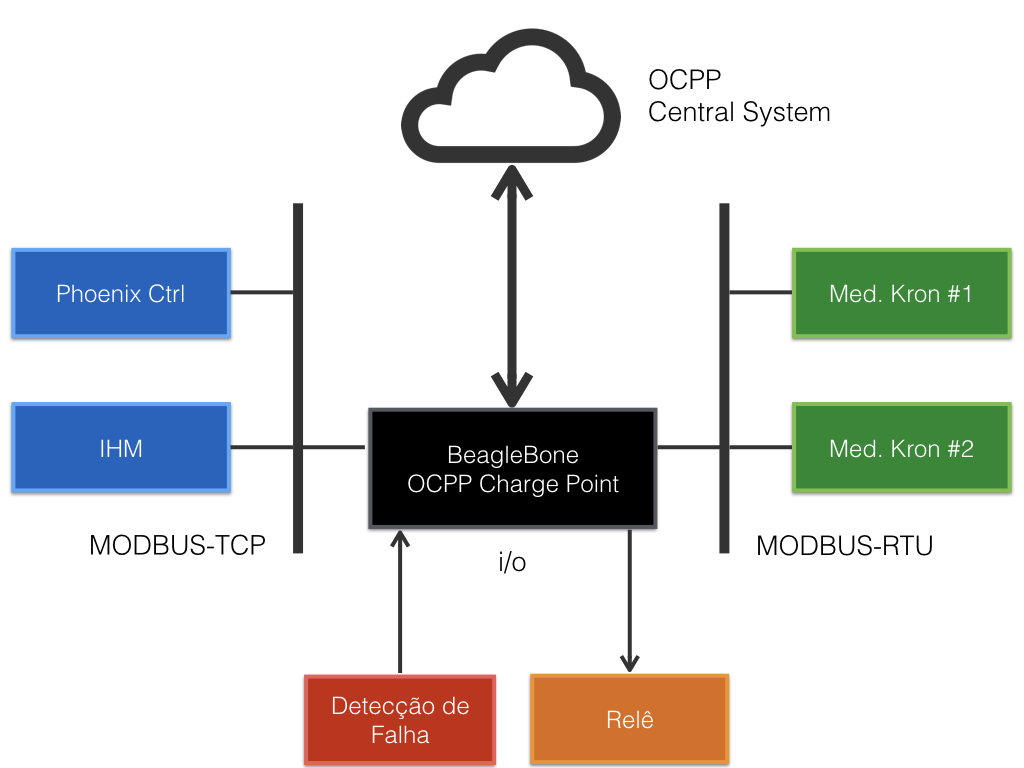
\includegraphics[width=0.8\textwidth,natwidth=400,natheight=288]{assets/images/devices-diagram.png}
        \caption{Diagrama de conexão entre os dispositivos da EVSE}
        \label{fig:proj-diagram}
      \end{center}
    \end{figure}

    \subsection{Especificações da estação}
    \label{methodology:structure:specs}

      O conector \textit{Mennekes} funciona em modo \ac{CA} trifásico, onde pode fornecer até 32 A sob tensão de 220 V (máxima corrente suportada pelo cabo utilizado). Devido a limitações, como corrente suportada pelo inversor do veículo ou nível de carga da bateria, a corrente consumida pode ser menor do que o limite dado pela estação, como é o caso do BMW i3, que utiliza apenas uma das fases do conector e utiliza somente até 25 A. 

      O outro conector, é uma tomada padrão ABNT padrão NBR 14136 \cite{nbr-14136} que pode fornecer até 20 A. Em carregamentos de carros, o cabo possui uma caixa de controle que se comunica com o veículo e controla a demanda de potência para o carregamento. Em alguns outros veículos, como bicicletas, o cabo possui também um inversor \ac{CA}-\ac{CC}, visto que o espaço nesses casos é reduzido.

    \subsection{Sistema operacional}
    \label{methodology:structure:os}

      O sistema que roda na BeagleBone é o Debian 8.6 (Jessie) com kernel \textit{Linux} específico para a \textit{BeagleBone}. Foi instalado o \textit{Java} e houveram modificações em sua \textit{device tree} para permitir a manipulação das entradas e saídas digitais.

      Foram adicionados alguns scripts no boot do sistema para ativar o acesso à internet e executar o programa logo após a inicialização do sistema.

    \subsection{Comunicação entre estação e servidores}
    \label{methodology:structure:ocpp}

      A estação implementa o protocolo \textit{\ac{OCPP}} 1.5, ao qual é suportado por outras estações comerciais vendidas no Brasil, permitindo comunicação com equipamentos e \textit{software} já existentes. A \textit{\ac{OCA}}, responsável pelo protocolo, disponibiliza um arquivo WSDL, onde é possível criar tanto um servidor quanto um cliente \textit{\ac{OCPP}} facilmente.

      Para a utilização desse arquivo em \textit{Java}, foi utilizada a ferramenta \textit{wsimport}. Essa ferramenta importa os arquivos e cria classes \textit{Java} correspondentes a cada \textit{endpoint}. Nem todas funções especificadas pelo protocolo foram implementadas, sendo que somente as da tabela \ref{table:ocpp} são suportadas.

      \begin{table}[]
        \centering
        \caption{Operações OCPP suportadas pela EVSE}
        \label{table:ocpp}
        \begin{tabular}{@{}ll@{}}
          \toprule
          \textbf{Enviada/Recebida} & \textbf{Operação}      \\ \midrule
            Enviada pela Estação      & BootNotification       \\
            Enviada pela Estação      & Heartbeat              \\
            Enviada pela Estação      & StartTransaction       \\
            Enviada pela Estação      & StopTransaction        \\
            Enviada pela Estação      & MeterValues            \\
            Enviada pela Estação      & StatusNotification     \\
            Enviada pela Estação      & Authorize              \\
            Recebida pela Estação     & RemoteStartTransaction \\
            Recebida pela Estação     & RemoteStopTransaction  \\
            Recebida pela Estação     & ChangeConfiguration    \\
            Recebida pela Estação     & GetConfiguration       \\
            Recebida pela Estação     & ChangeAvailability     \\ \bottomrule
        \end{tabular}
      \end{table}

    \subsection{IHM}
    \label{methodology:structure:others}

      O software da \ac{IHM} não foi desenvolvido pelo acadêmico, porém são de importância fundamental para o projeto. A escolha das telas foi realizada em equipe e implementada no software \textit{EasyBuilder 2000}. {}

      A interface é atualizada a cada 200 milissegundos para evitar dados desatualizados ou respostas lentas à entradas do usuário. Ainda assim foram observados atrasos, ligados a capacidade de processamento da \ac{IHM} com requisições muito frequentes a seus registradores. A comunicação e gerenciamento da \ac{IHM} se dá pelo \textit{HmiManager}, apresentado na seção \ref{methodology:structure:sw}.

  \section{Software}
  \label{methodology:structure:sw}

    \subsection{Principais Classes}

    Devido a complexidade do projeto de software e suas diversas classes e implementações, a lista abaixo resume as principais classes que permitem o funcionamento da estação. Essas serão referidas nas seguintes seções sobre o funcionamento da estação. 

        \subsubsection{AuthHandler}
          Gerencia autenticação via \textit{\textit{\ac{RFID}}}. Primeiramente verifica se o usuário está habilitado por meio de uma \textit{whitelist} e, caso não encontre nenhum dado nela, faz uma requisição ao servidor \textit{\ac{OCPP}} para a verificação.
        \subsubsection{OcppManager}
          Roda em uma instância própria e, a cada período de tempo, executa a lista de comandos que foram criados pelo programa. Implementa o \textit{Dispatcher} do \textit{Command Pattern} \cite{book-gof}, onde os seus comandos são implementações das requisições da tabela \ref{table:ocpp}, e roda em uma instância individual.
        \subsubsection{ChargePointServer}
          Implementação da interface \textit{\ac{WSDL}} gerada pelo \textit{wsimport}. Roda em uma instância individual e cria um servidor ao qual o \textit{Central System} pode requisitar dados.
        \subsubsection{ChargePointClient}
          Implementação da interface \textit{\ac{WSDL}} gerada pelo \textit{wsimport}. Permite enviar requisições para o \textit{Central System} e é chamado apenas por comandos despachados pelo \textit{OcppManager}.
        \subsubsection{HmiManager}
          Gerencia os estados da \ac{IHM}, sendo que todos estados são representados por classes. Implementa o \textit{Context} do \textit{State Pattern} \cite{book-gof}, sendo que cada estado (implementações da classe \textit{ScreenState}) pode modificar qual será o estado da próxima iteração por meio de informações adquiridas do dispositivo \ac{IHM} ou de dados vindos de outras dependências. Roda em uma instância própria.
        \subsubsection{ConnectorSupervisor}
          Roda em uma instância, onde checa periodicamente o status dos conectores, envia informações para o servidor sobre dados de medição destes e expira antigas reservas (esse último será implementado em versões futuras).
        \subsubsection{ConnectorManager e Connector}
          Classe que armazena todos conectores, sendo cada conector um objeto \textit{Connector}. As classes \textit{Connector} gerenciam cada conector da estação, o que possibilita a obtenção de dados e controle por meio de diferentes interfaces (\ac{IO} e MODBUS no momento).
        \subsubsection{TransactionManager e Transaction}
          Classe que armazena transações ativas, sendo que transações são instâncias da classe \textit{Transaction}. Cada transação roda em uma instância individual, sendo que estas são responsáveis pelos processos de inicialização e finalização junto ao \textit{\ac{OCPP}}, assim como envio periódico de dados da transação.

    \subsection{Inicialização}

      A figura \ref{fig:sw-init} apresenta como o programa é inicializado. Deve-se levar em conta que a primeira coisa a ser executada, antes mesmo da sequência definida no \textit{main()}, é a inicialização do \textit{Guice}, onde todos \textit{check-ups} iniciais são feitos para verificar se não há nenhuma declaração errada em sua configuração.

      \begin{figure}[H]
        \begin{center}
          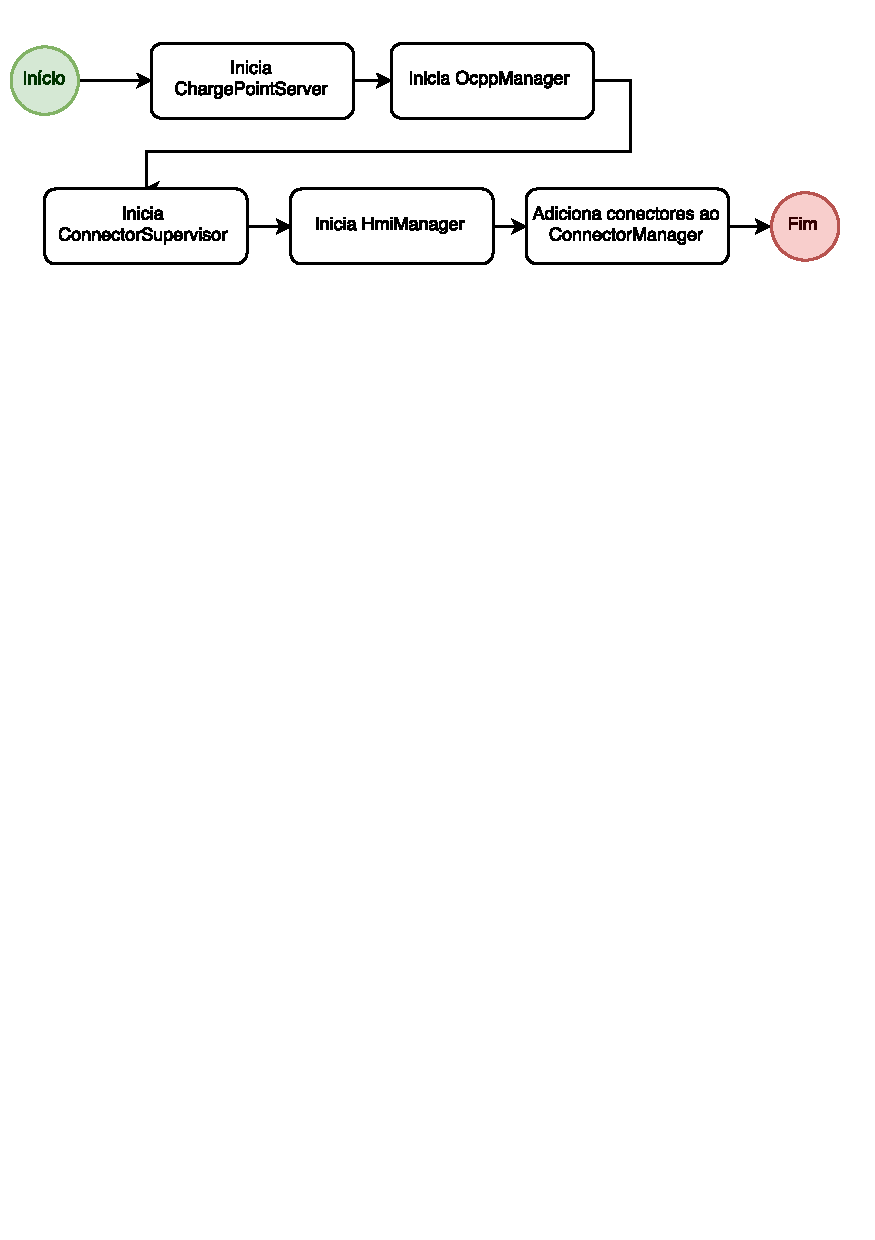
\includegraphics[width=\textwidth]{assets/pdfs/sw-init.pdf}
          \caption{Sequência de Inicialização}
          \label{fig:sw-init}
        \end{center}
      \end{figure}

      Todas classes que são instâncias independentes são inicializadas, menos a classe \textit{Transaction} que só é inicializada quando há uma transação à ser iniciada. Visando prover agilidade, as configurações dos conectores são declaradas no corpo da classe que contém o \textit{main()}, porém foi observado que poderia ser criada uma classe que adquirisse os dados da configuração do conector (atualmente em \textit{settings.properties}) e adicionasse esses conectores ao \textit{ConnectorManager}.

    \subsection{Inicialização e Finalização de Transações pelo Usuário}

      Para inicializar uma transação (carregamento), o usuário precisa ser registrado no sistema, sendo que este é validado por meio de uma \textit{tag \ac{RFID}}. A figura \ref{fig:sw-starttransaction} demonstra o processo que o usuário deve executar para inicializar a transação com uma \textit{tag RFID}.

      Após encostar a \textit{tag} no leitor, o \textit{HmiManager} chama o \textit{AuthHandler} para verificar se o usuário está ou não habilitado para carregar veículos na estação. Caso não, uma mensagem de erro é exibida e a \ac{IHM} retorna para a tela inicial.

      Após autenticar, o usuário precisa escolher um dos conectores disponíveis. Assim que escolhido, o \textit{HmiManager} chama o \textit{TransactionManager}, ao qual se encarrega de inicializar uma transação (\textit{Transaction}). Ao inicializar a transação, uma \textit{Thread} é criada. A primeira tarefa desta é habilitar o carregamento, chamando a classe \textit{Conector} relacionada para tal. Por fim, o servidor \ac{OCPP} é notificado da transação e o usuário recebe uma mensagem notificando que seu carregamento foi iniciado.

      Também é possível inicializar uma transação por meio de um aplicativo. Nesse caso, o servidor OCPP mandará uma \textit{RemoteStartTransaction}, que iniciaria o mesmo processo como se fosse uma \textit{tag RFID}, porém feito por meio de um servidor e não fisicamente.

      A finalização de um carregamento é dada basicamente da mesma maneira e é apresentada na figura \ref{fig:sw-stoptransaction}. Uma das diferenças é que, após o usuário ser autenticado, é checado se ele possui uma transação ativa. Caso houver, aparecerá o conector que ele pode cancelar o carregamento. Os outros processos são o inverso da inicialização (para a \textit{Thread} e desabilita carregamento).

      Um carregamento pode também ser finalizado pelo \textit{ConnectorSupervisor}, de forma automática, nos seguintes casos: 

      \begin{itemize}
        \item Alguma falha durante o carregamento
        \item Conector desconectado do veículo por parte do usuário
        \item Carregamento ter chego ao fim (consumo próximo de zero)
      \end{itemize}

      \begin{figure}[H]
        \begin{center}
          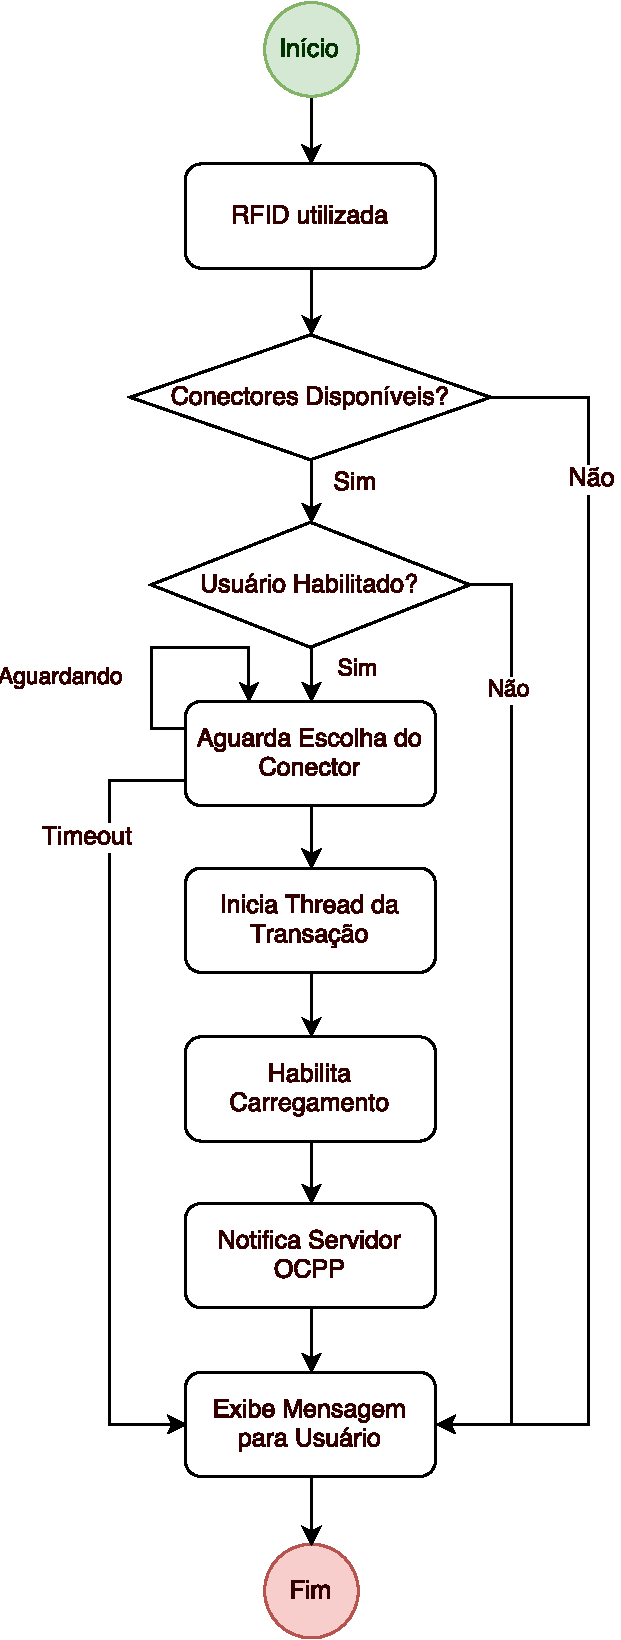
\includegraphics[height=\textheight]{assets/pdfs/sw-starttransaction.pdf}
          \caption{Diagrama de Inicialização de uma Transação pelo usuário}
          \label{fig:sw-starttransaction}
        \end{center}
      \end{figure}

      \begin{figure}[H]
        \begin{center}
          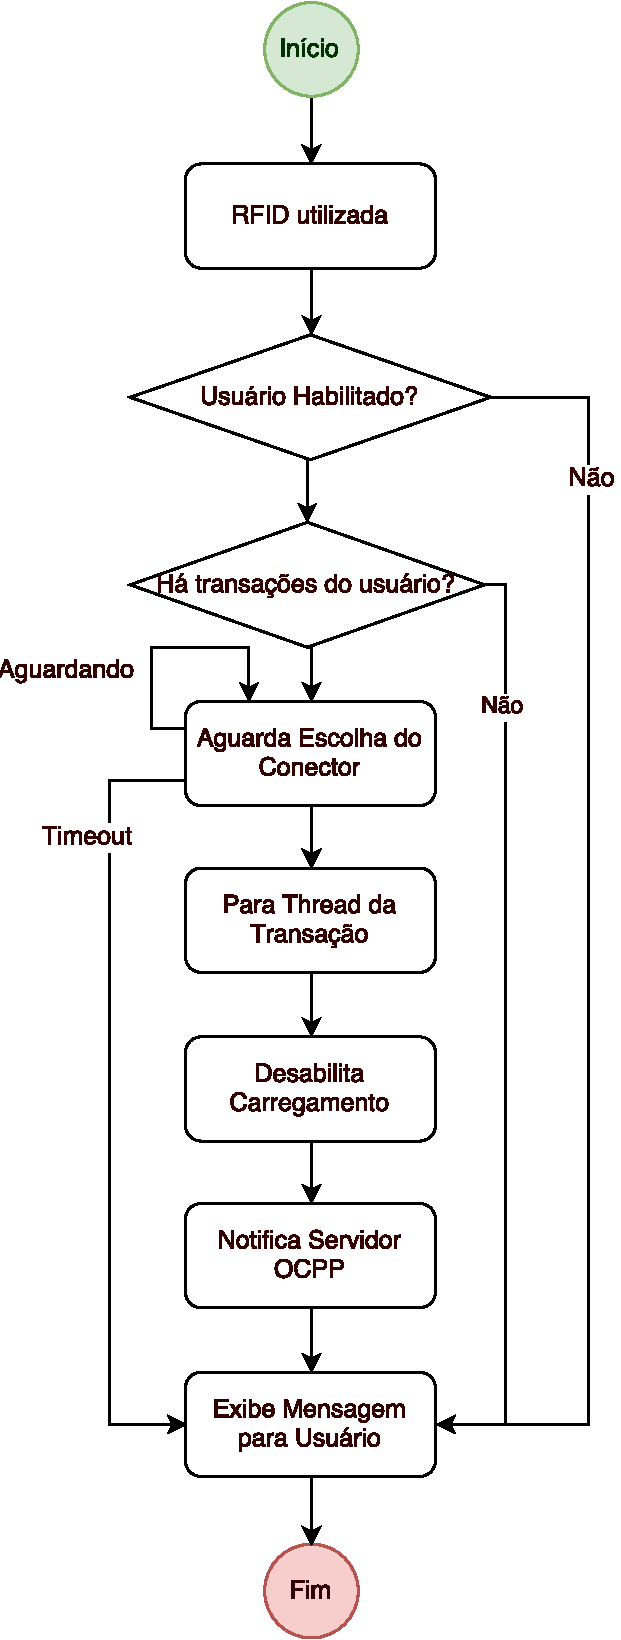
\includegraphics[height=\textheight]{assets/pdfs/sw-stoptransaction.pdf}
          \caption{Diagrama de Finalização de uma Transação pelo usuário}
          \label{fig:sw-stoptransaction}
        \end{center}
      \end{figure}
